\newpage
\section{Tổng quan về hệ thống}


Trong thời đại công nghệ hiện nay,
việc ứng dụng công nghệ vào cuộc sống trở thành một phần không thể thiếu.
Đặc biệt trong thời đại công nghệ trí tuệ nhân tạo (AI) đang bùng nổ.
Mục tiêu của ứng dụng này là
phát triển một hệ thống hỏi đáp về pháp luật Việt Nam.
Việc ứng dụng công nghệ AI
đánh dấu sự chuyển dịch lớn của ngành pháp lý
từ sử dụng các công cụ, phương thức tìm kiếm thủ công
sang hệ thống xử lý ngôn ngữ tự nhiên (NLP).
Việc ứng dụng công nghệ xử lý ngôn ngữ tự nhiên
giúp máy tính hiểu và xử lý được ngôn ngữ của con người.


\subsection{Sự cần thiết}


Hệ thống tài liệu văn bản pháp luật rất phức tạp.
Sự phức tạp không chỉ nằm ở khối lượng dữ liệu,
mà các văn bản có thể thay thế, bổ sung, hết hiệu lực, \dots
Trong một số trường hợp một văn bản vừa hết hiệu lực
hoặc bị thay thế
thì con người có thể chưa kịp cập nhật thông tin.
Đặc biệt là đối với những người bận rộn.
Từ đó, có thể dẫn đến những sai sót, thậm chí là thiệt hại về tài chính và rủi ro pháp lý.


\begin{figure}[H]
   \centering
   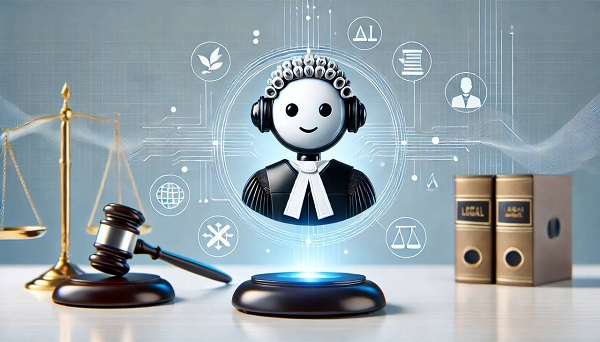
\includegraphics[scale = 0.9]{pictures/chatbot-tra-cuu-luat-la-gi.jpeg}
   \caption{AI hỗ trợ tư vấn pháp luật}
\end{figure}


Đối với ứng dụng AI thì sẽ có các điểm mạnh như sau:


\begin{itemize}


   \item         Tiết kiệm chi phí
   \item         Hoạt động làm việc 24/7
   \item         Phản hồi nhanh chóng
   \item         Cập nhật thông tin thường xuyên
   \item         Trích dẫn thông tin chi tiết


\end{itemize}


Vì AI phụ thuộc vào dữ liệu đầu vào,
do việc cập nhật dữ liệu không được ngay lập tức,
nên không đảm bảo tính chính xác của các văn bản pháp luật
dẫn đến hạn chế và thách thức về độ chính xác của ứng dụng.
Vì vậy, trong môi trường đòi hỏi sự chính xác tuyệt đối như pháp luật
thì công cụ AI chỉ đóng vai trò trợ lý hỗ trợ, nguồn tham khảo và không thể thay thế con người.
Do đó, để sử dụng AI hiệu quả và tránh những rủi ro sai lệch thông tin,
người dùng phải kiểm chứng thông tin với chuyên gia và các CSDL chính thống trong các vấn đề mang tính quyết định quan trọng.


\subsection{Khảo sát công nghệ xây dựng}
\subsubsection{Mô hình ngôn ngữ lớn}


Năm 2017, các kỹ sư của Google
đưa ra bài báo "Attention Is All You Need"
khai sinh kiến trúc Transformer
với cơ chế Self-Attention (Tự chú ý),
mở đường cho hầu hết kiến trúc
LLM (Large Language Model) hiện nay.

Cách hoạt động của LLM
là dự đoán xác suất của từ tiếp theo
dựa theo các từ đã xuất hiện trước đó.


Ví dụ:


\begin{figure}[H]
   \centering
   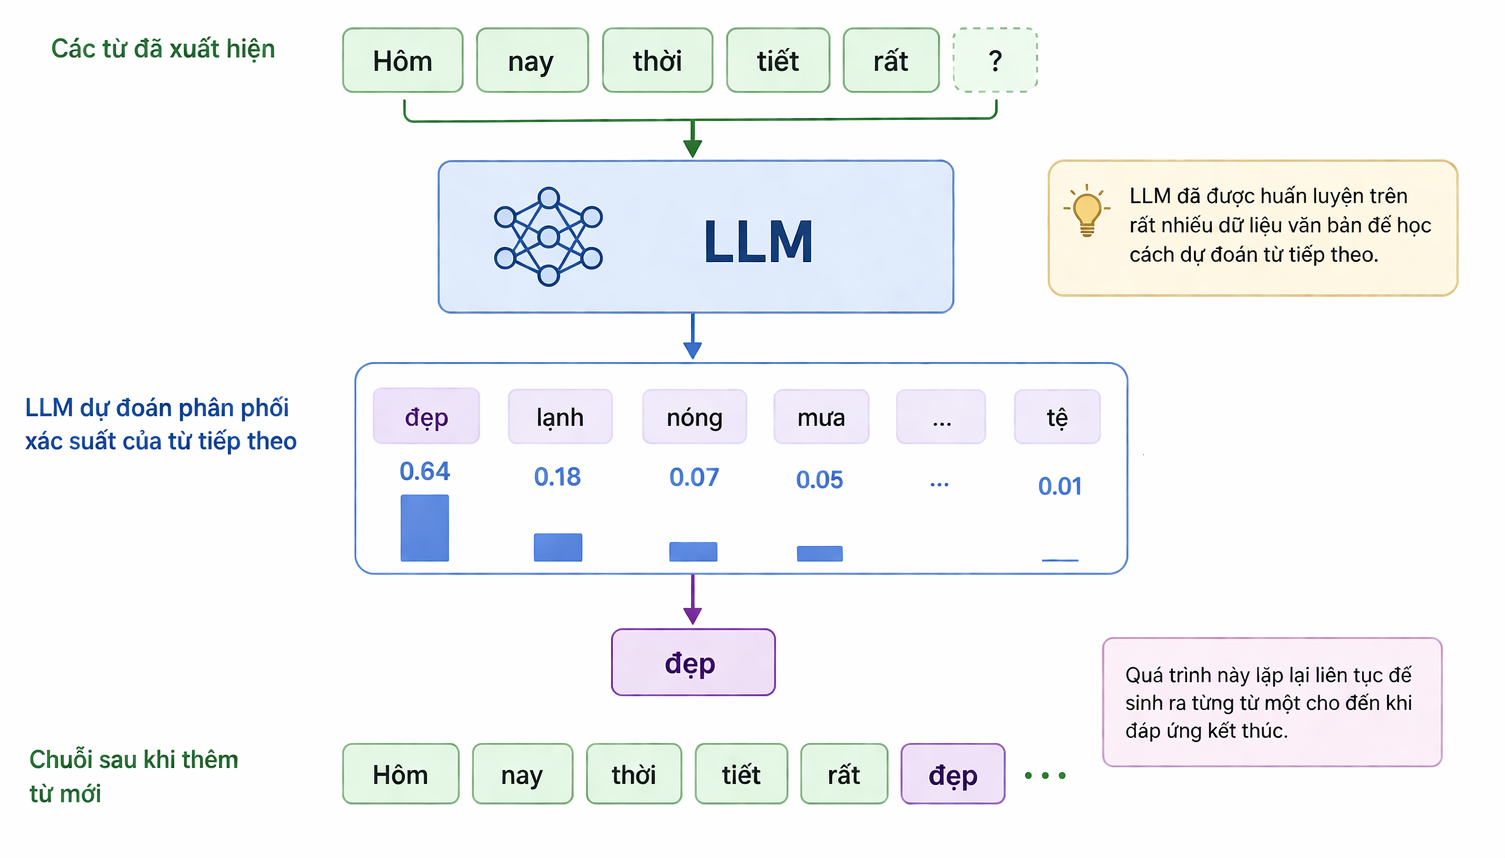
\includegraphics[scale = 0.4]{pictures/llm.png}
   \caption{Cách hoạt động của LLM}
\end{figure}

Tuy nhiên LLM có một số nhược điểm:


\begin{itemize}


   \item  Dữ liệu huấn luyện rộng

   \item  Độ chính xác không cao với miền cụ thể

   \item  Có hiện tượng ảo giác (Hallucination)

   \item  Dữ liệu chỉ cập nhật đến ngày train, dữ liệu cũ

   \item  LLM không biết dữ liệu mới

   \item  LLM không biết dữ liệu doanh nghiệp

   \item  LLM không biết tài liệu người dùng

   \item  Chi phí cho việc huấn luyện, tinh chỉnh lớn.


\end{itemize}


\begin{figure}[H]
   \centering
   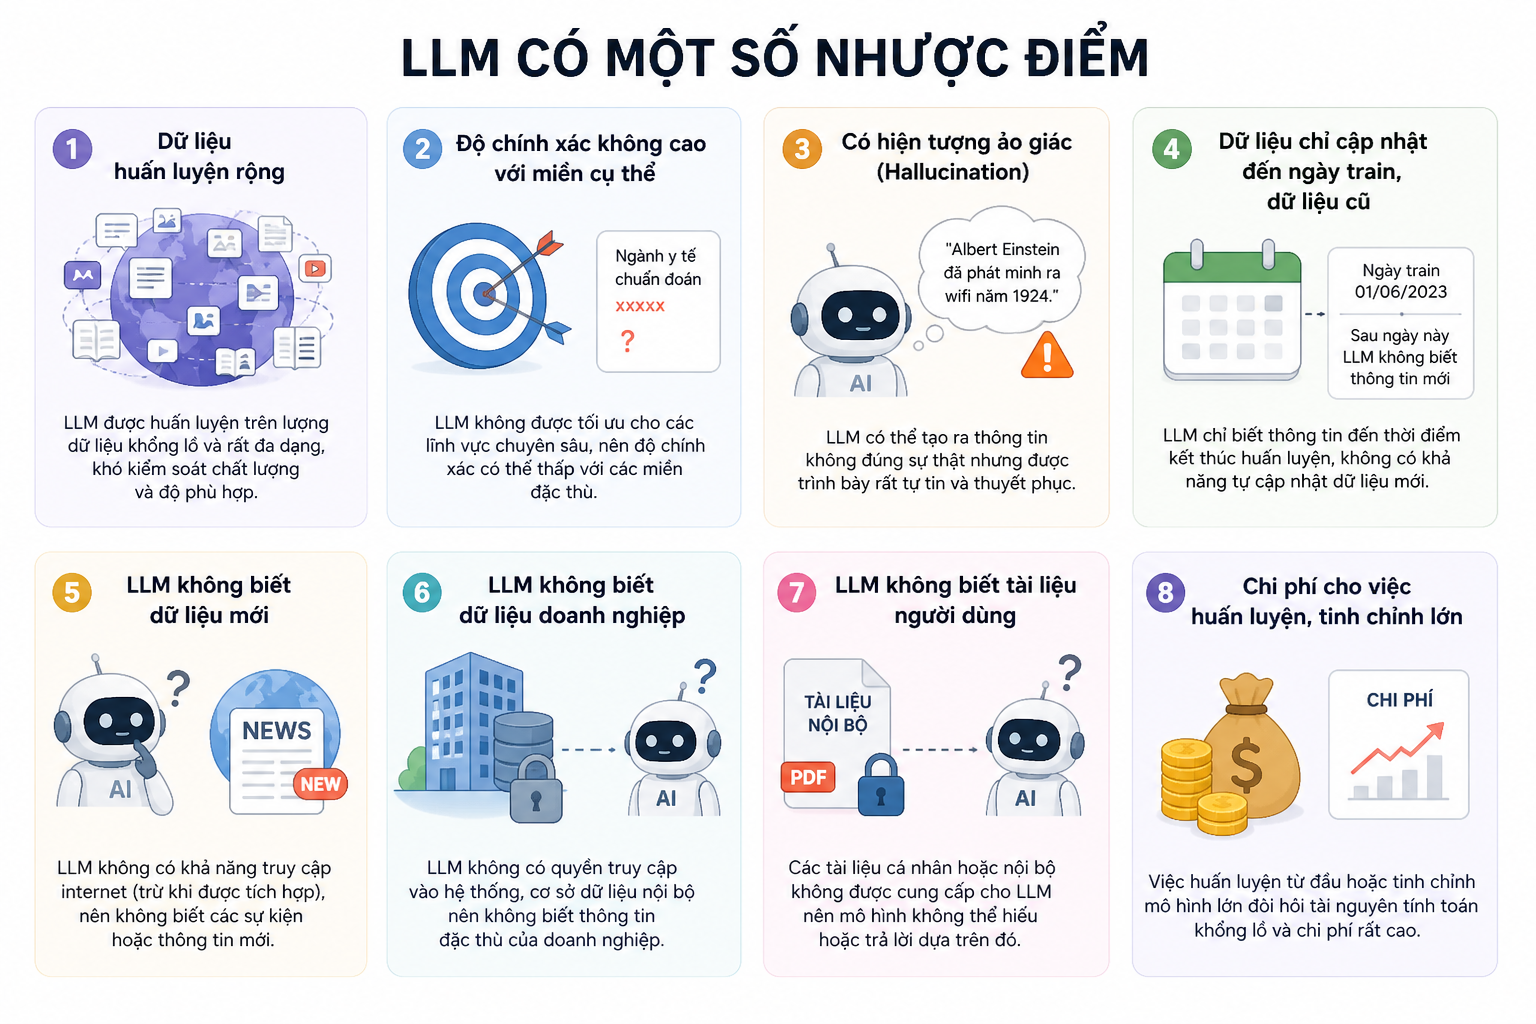
\includegraphics[scale = 0.25]{pictures/llm-crons.png}
   \caption{Một số nhược điểm của LLM}
\end{figure}


\subsection{Mục tiêu}
